% !TEX program = pdflatex
% radcoolpv: how to run the code on macOS vs. Google Colab.
% Standalone, tightly cropped vector PDF. Native width ~123mm so it drops
% into the host manual's 130mm text column at scale ~1 -- font sizes are
% chosen at that final width, not scaled after the fact.
\documentclass[11pt, tikz, border=2pt]{standalone}

\usepackage[T1]{fontenc}
\usepackage{libertinus}          % match the host manual's body font
\usetikzlibrary{arrows.meta, calc, positioning}

% --- Palette: black + gray + one accent (Okabe-Ito blue). CVD- and
%     grayscale-safe; the accent marks the one claim this figure makes: both
%     paths drive the identical three-stage pipeline.
\definecolor{accent}{HTML}{0072B2}
\definecolor{ctxgray}{gray}{0.45}

\newcommand{\code}[1]{\texttt{#1}}
\newcommand{\ann}[1]{\\[1pt]{\footnotesize\color{ctxgray}#1}}

\begin{document}
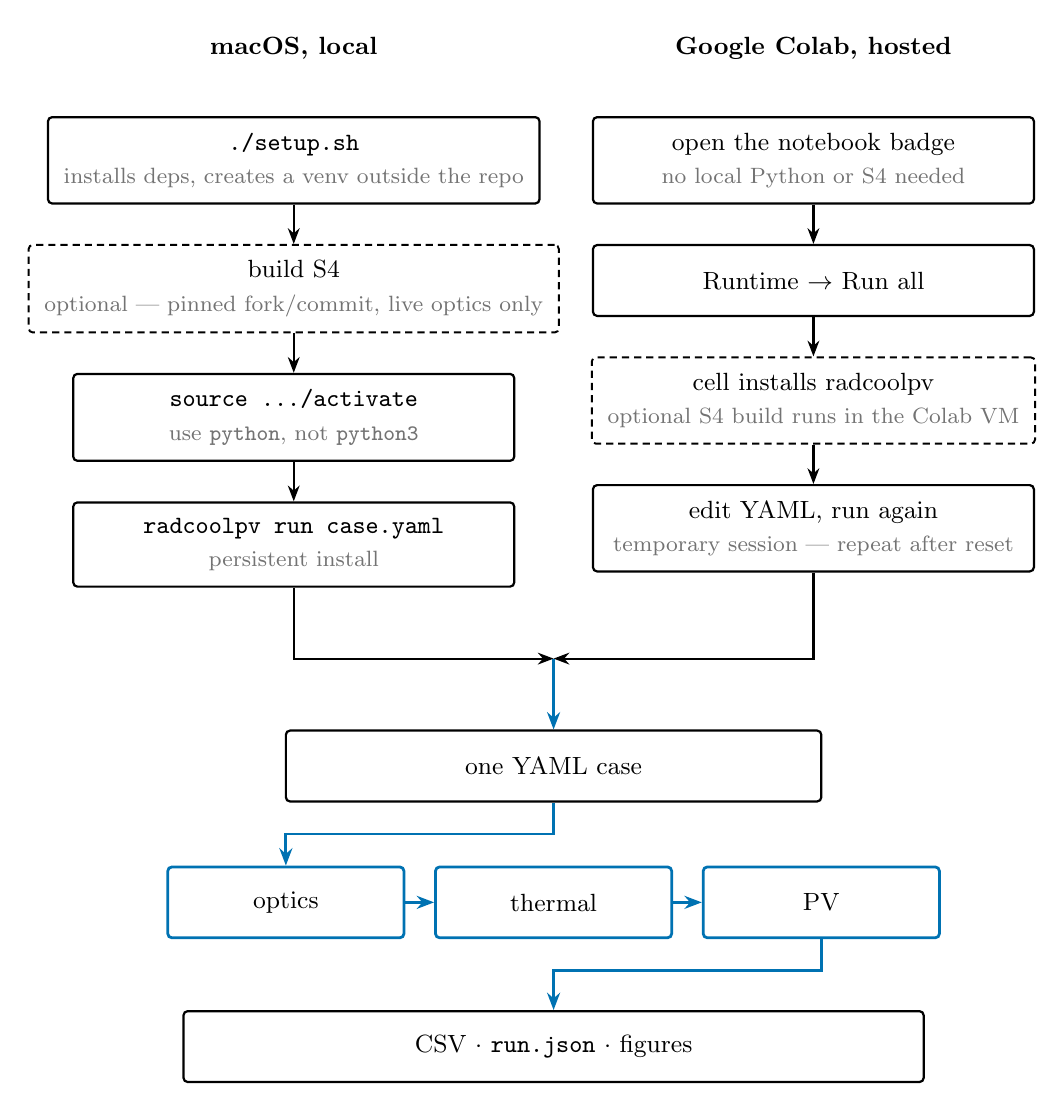
\begin{tikzpicture}[
  every node/.style = {font=\small},
  colhead/.style   = {font=\small\bfseries, align=center},
  boxstep/.style   = {draw=black, line width=0.8pt, rounded corners=1.5pt,
                       align=center, minimum width=56mm, minimum height=9mm,
                       inner sep=2mm, font=\small},
  optstep/.style   = {boxstep, dash pattern=on 2.6pt off 1.8pt, line width=0.7pt},
  flow/.style      = {-{Stealth[length=2mm]}, draw=black, line width=0.8pt},
  accentflow/.style= {-{Stealth[length=2.2mm]}, draw=accent, line width=1pt},
  pipebox/.style   = {draw=accent, line width=1pt, rounded corners=1.5pt,
                       align=center, minimum width=30mm, minimum height=9mm,
                       inner sep=1mm, font=\small},
  outbox/.style    = {draw=black, line width=0.8pt, rounded corners=1.5pt,
                       align=center, minimum width=94mm, minimum height=9mm,
                       font=\small},
]

  % ---------------------------------------------------------------- headers
  \node[colhead]                    (h1) at (-33mm,0) {macOS, local};
  \node[colhead]                    (h2) at (33mm,0)  {Google Colab, hosted};

  % ------------------------------------------------------------- macOS path
  \node[boxstep, below=6mm of h1]  (m1) {\code{./setup.sh}
        \ann{installs deps, creates a venv outside the repo}};
  \node[optstep, below=5mm of m1] (m2) {build S4
        \ann{optional --- pinned fork/commit, live optics only}};
  \node[boxstep, below=5mm of m2]  (m3) {\code{source .../activate}
        \ann{use \code{python}, not \code{python3}}};
  \node[boxstep, below=5mm of m3]  (m4) {\code{radcoolpv run case.yaml}
        \ann{persistent install}};

  % ------------------------------------------------------------ Colab path
  \node[boxstep, below=6mm of h2]  (c1) {open the notebook badge
        \ann{no local Python or S4 needed}};
  \node[boxstep, below=5mm of c1]  (c2) {Runtime \(\to\) Run all};
  \node[optstep, below=5mm of c2] (c3) {cell installs radcoolpv
        \ann{optional S4 build runs in the Colab VM}};
  \node[boxstep, below=5mm of c3]  (c4) {edit YAML, run again
        \ann{temporary session --- repeat after reset}};

  % --------------------------------------------------------------- linkage
  \draw[flow] (m1) -- (m2);
  \draw[flow] (m2) -- (m3);
  \draw[flow] (m3) -- (m4);
  \draw[flow] (c1) -- (c2);
  \draw[flow] (c2) -- (c3);
  \draw[flow] (c3) -- (c4);

  % --------------------------------------------------------------- merge
  \path let \p1=(m4.south), \p2=(c4.south) in
        coordinate (joinM) at (0, {min(\y1,\y2) - 9mm});
  \draw[flow] (m4.south) |- (joinM);
  \draw[flow] (c4.south) |- (joinM);

  \node[boxstep, below=9mm of joinM, minimum width=68mm] (yaml) {one YAML case};
  \draw[accentflow] (joinM) -- (yaml.north);

  % ----------------------------------------------------------- pipeline
  \node[pipebox, below=8mm of yaml, xshift=-34mm] (opt) {optics};
  \node[pipebox, below=8mm of yaml]               (th)  {thermal};
  \node[pipebox, below=8mm of yaml, xshift=34mm]  (pv)  {PV};
  \draw[accentflow] (yaml.south) -- ++(0,-4mm) -| (opt.north);
  \draw[accentflow] (opt) -- (th);
  \draw[accentflow] (th) -- (pv);

  \node[outbox, below=9mm of th] (out) {CSV \(\cdot\) \code{run.json} \(\cdot\) figures};
  \draw[accentflow] (pv.south) -- ++(0,-4mm) -| (out.north);

\end{tikzpicture}
\end{document}
